\chapter{Physics performance}
\label{Chapter:Higgs}

\section{Introduction}
\subsection { Higgs discovery and Physics at Post-Higgs era }
The discovery of the Higgs boson in 2012 is a historic event in the  fundamental physics research.
This discovery certainly represents the summit of the success of the Standard Model (SM),
in the sense that the entire SM particle spectrum has been completed.
However, profound break through are still required to fully understand the SM and the underlying fundamental physics principles. 

The SM itself is in an extremely interesting position.
First of all, the SM is certainly one of the most successful models that mankind have ever constructed,
in the sense that the SM matches perfectly the experimental data taken at all the collider physics.
However, outside the collider laboratories, the SM is incapable to explain lots of the fundamental and extremely important phenomena,
such as the dark matter, dark energy and the baryon asymmetry.
In addition, the SM has lots of theory defects, in the sense that it is characterized by a series of coincidence,
for example, the SM predicts the vacuum is in a meta-stable state,
the SM explains the Higgs boson mass as a cancellation of two big numbers with the precision of $10^{40}$, {\it etc}. 

Interesting though, most of the theory defects and possibly many
of the unexplained fundamental phenomena are correlated with the Higgs boson.
The Higgs boson itself represents the Naturalness problem;
the couplings between Higgs bosons and the fermions inhabit the CP violation phases.
A second order phase transition of the Higgs field during the SSB is required to preserve the baryon asymmetry.
The Higgs boson may serves as a portal to the dark matter and even dark energy.
In this sense, the Higgs boson itself is an extremely sensitive,
maybe even the best probe towards the fundamental physics principles underlying the SM. 

In this sense, a better understanding of the Higgs boson,
the Higgs mechanism and the direct search for new physics
beyond the stand model certainly becomes the focus of the experimental particle physics after the Higgs discovery.
Precise Higgs factories therefore become a must for the particle physics and fundamental physics researches,
with which we can explore through the probe of the Higgs boson.

In terms of the precision measurement, better accuracy means better physics reaches ...

The LHC is a power Higgs factory. It not only discovers the Higgs boson,
but could also determine the Higgs boson properties to a great precision,
especially with the anticipated 3 ab$^{-1}$ of integrated luminosity by the HL-LHC.
However, the Higgs boson property measurements at the LHC are largely limited by the huge QCD background,
and the fact that most of the Higgs signal can only be determined from a direct reconstruction of the Higgs boson decay final state.
As a result, a extremely small fraction (roughly $10^{-3}$) of the Higgs events can actually be recorded at the LHC,
and the Higgs measurement precision (in terms of the signal strength),
is limited to roughly 10\% level;
with which the LHC could shed light on the new physics close to the TeV scale. 

The electron positron collider provides crucial information on top of the proton colliders.
First of all, the electron positron Higgs factory is free of the QCD background.
The ratio between the cross section of the Higgs events
and the inclusive Physics events within the detector fiducially volume is roughly $10^{-2} \sim 10^{-3}$,
roughly eight orders of magnitude better than that at the proton colliders.
In fact, the entire event rate at an electron positron collider is so low
that it's feasible to operate the detector in a triggerless mode
and record all the physics event for the off-line analysis --- with which almost all the Higgs signals will be recorded.
In addition, a significant portion of the Higgs boson is generated together with a $Z$ boson
through the $s$-channel Higgsstrahlung process,
with which the Higgs boson could be identified through the $Z$ boson via the recoil mass method,
therefore, the inclusive $ZH$ cross section can be measured model independently,
which leads to absolute measurements of the Higgs boson width and couplings to between Higgs boson decay final states.
Meanwhile, the electron positron colliders are extremely sensitive to the exotic Higgs decay mode search. 

For these very advantages, many Electron Positron Higgs factories have been proposed [].
The fact that the Higgs boson has a mass of 125 GeV promotes the idea of a circular collider,
which could be upgraded from high precision electron positron collider to a high-energy proton collider.
Based on these considerations, the Chinese high-energy physics community proposed the Circular Electron Positron Collider (Project).
In the currently design, the CEPC will be installed in a tunnel with total circumference of 100 km;
as a Higgs factory, it will be operated at 240 GeV center of mass energy
and deliver 1 Million Higgs boson in 10 years operation with two detectors.
At this energy, roughly 95\% of the Higgs bosons are generated via the ZH process,
ensuring an excellent $g(HZZ)$ measurement.
Lowing the center of mass energy to 91.2 GeV, the CEPC could produce $10^{10}$ $Z$ boson in 1 year operation.
After the electron positron collider,
a super proton proton collider (SppC) with center of mass energy at 100 TeV could be installed in the same tunnel,
which could also be used to perform heavy ion collisions.
The utilization of a large radius tunnel and careful over-all design should in principle reserve the possibility of $e-p$ collider. 

In terms of Higgs measurement, the CEPC could determine the absolute Higgs couplings to percentage-permille level accuracy.
In terms of the Higgs signal strength measurement, the CEPC would have a precision at least 1 order of magnitude superior
than that of the HL-LHC.
The Higgs total width, which can only be determined to a relative accuracy of ~40\% with model dependent assumptions at the HL-LHC,
could be measured to percentage level accuracy at CEPC.
The exotic decay branching ratios could be limited to $10^{-3}$ to $10^{-6}$,
depends on the signal topology.
Meanwhile, the CEPC also produces lots of $Z$ and $W$ bosons with precisely known initial state,
with which the EW precision measurement could also be improved by at least one order of magnitude comparing
to the current experiment reaches. 

It should also be mentioned that the electron positron collider
and the proton colliders provides complementary description of the Higgs boson properties.
In addition, a combination of the precise EW measurement
and the Higgs measurement would largely increase the sensitivity of new physics reaches, in the context of EFT [XXX].  

In one word, the CEPC-SppC project provides a combination of high precision measurements and the high-energy frontier,
aiming at the core physics program after the Higgs discovery,
and an intensive physics program with total duration of several decades up-to half a century.


\subsection { The physics requirement and detector design at the CEPC }

Most of the Higgs events could be recorded at the electron positron collider.
These Higgs events have various different topologies, given the fact that Higgs boson could be generated with,
and decay into various physics objects.
Therefore, the detector at an electron positron Higgs factory should be able to distinguish
not only the Higgs signal from the SM background,
but also the Higgs signal in between its different generation mode and decay final states.
In other word, the CEPC detector should be able to reconstruct the key physics objects,
i.e, photons, leptons, taus, jets and missing energy/momentum, at high efficiency,
high purity and high precision. Explicitly, the physics requirements to the CEPC detector could be schematized as: 

\begin{itemize}
\item []1, Be adapted to the CEPC collision environment;
\item []2, Have large solid angle coverage;
\item []3, Provide excellent lepton identification;
\item []4, The Track should have excellent track reconstruction efficiency and
  a resolution better than $\delta(\frac{1}{P_t}) = 2\times 10^{-5}(\mbox{GeV}^{-1})$;
  the latter is required by $Br(H \to\mu^+\mu^-)$ measurement at the CEPC;
\item []5, Precise reconstruction of photons, requested by both jet energy reconstruction and the $Br(H\to \gamma\gamma)$ measurement;
\item []6, Capability to separate charged kaons from pions, which enables an excellent flavor physics program at CEPC;
\item []7, Good Jet/MET reconstruction;
\item []8, Capability of separate $b$-jets, $c$-jets and light jets: requested by $g(Hbb)$, $g(Hcc)$, and $g(Hgg)$ measurements.
\end{itemize}

The detector requirement for the EW measurements should be in principle similar to these at the Higgs runs.
Meanwhile, the majority of EW measurements at the CEPC would be limited by the systematic, thus,
the detector for the EW measurements should also has excellent alignment, calibration and stability,
to control the systematic at the CEPC EW measurements.
In addition,
the CEPC should provide $10^{-3}$ luminosity monitoring at Higgs operation and $10^{-4}$ luminosity measurement at $Z$ pole operation.
Ideally, the beam energy is required to be calibrated to 1 MeV level for the EW measurement. 

Nowadays, with the progress of micro-electronics,
the particle flow oriented detector design has became a clear trend for the collider detector design[CMS, ATLAS, CALICE].
A Particle Flow oriented detector aims at reconstruct all the final state particles, with the most suited sub-detector system.
The physics objects are then reconstructed from the final state particles.
The Particle Flow Algorithm, at an adequate detector design,
could significant enhance the reconstruction performance all the physics objects,
and largely improve the accuracy of jet energy resolution, since the majority of jet energy is stored in the charged hadrons,
whose momentum is usually measured with a much better accuracy than its cluster energy to be measured at the calorimeter system. 

Detector-wise, the Particle Flow oriented detector design appreciates precise tracking system
with limited material budget and a limited dead space among different sub-detectors.
Low-material tracker is required to limit the probability of interactions before the particle reach the calorimeter,
i.e, via multi-scattering, bremsstrahlung and hadron-nuclear interactions.
A high granularity calorimeter system is the key component of a PFA oriented detector design,
since the calorimeter would be response to separate all the final state particle showers in the calorimeter,
and provide essential information for the lepton identification accordingly. 

% In one word, a successful detector design arises with respect to the principle of maximize the recorded information and a reliable interpretation of all the detector signal. 

A PFA oriented detector concept has been established as the benchmark detector design for the CEPC physics studies.
The detector geometry is initialized on the ALEPH, SiD and ILD detector geometry,
and the geometry parameters are determined via a series of the detector optimization studies.
On the other hand, a dedicated PFA reconstruction algorithm, Arbor,
aiming at a precise interpretation of the general detector signals, has been developed.
The combination of CEPC benchmark detector and the Arbor algorithm provides precise reconstruction of all the physics objects,
with which the CEPC physics potential has been demonstrated on a series of the full simulation analyses.
We would like to summarize the reconstruction performance of this combination,
at both individual physics object level as well as at Higgs physics benchmark level, in this very manuscript. 

This manuscript is organized as following.
The detector geometry and simulation details are introduced in section 2.
Section 3 is devoting to the architecture and core algorithms of the Arbor algorithm.
From Section 4 to section 7, we will demonstrate the particle flow reconstruction performance at CEPC:
the reconstruction of leptons, photons, taus, jets, missing energy and missing momentums will be discussed intensively, respectively.
In section 8, we will summarize this manuscript. 

\section{ Simulation Geometry \& Samples }

A particle flow oriented detector concept, PICARDO, has been established as the benchmark detector model for the CEPC CDR study.
This geometry is developed from ALEPH detector, SiD concept, and most importantly, the ILD concept.
To get adequate to the CEPC collision environment, the PICADO geometry has dedicated MDI \& Forward region design.
Feasibility studies have been operated for the main Tracker and Calorimeter,
from which we conclude the detector could be operated at Z pole runs with physics event rate of 1 k Hz.
The major detector parameters, i.e, the size of tracker, the thickness of calorimeter, {\it etc},
are optimized towards a set of benchmark physics processes, covering all key physics objects []. 

To fulfill the physics requirement of the CEPC and to be optimized towards the Particle Flow Reconstruction,
the PICADRO uses low material tracking system, ultrahigh granularity calorimeter system and a large,
3-Tesla B-Field that can host the entire ECAL and HCAL inside. 


The tracking system includes a TPC main tracker,
a Silicon Pixel Vertex System, and the Silicon Forward/External Tracking system based on silicon strip technology. 

The TPC has an inner radius of 330 mm and an outer radius of 1800 mm.
The TPC is divided into 220 radical layers with layer thickness of 6 mm,
each layer is then divided into 1 mm cells along the phi-direction.
The TPC will have 10 million readout channels in each side of the endcap,
each channel with an intrinsic spatial resolution of 100 $\mu$m
in $R-\phi$ direction and 500 $\mu$m resolution in the $Z$ direction.
Such configuration provides providing large number of spatial point for track finding.

The basic geometry parameter and performance is listed in Table XX. 


A successful detector ... 

The in-homogeneity and geometry defects may caused a significant degrading towards the neutral object reconstruction,
i.e, the photons and the neutral hadrons in the jet.
To understand this effect, a simplified calorimeter with cylindrical barrel layers has been implemented.
To first order, this simplified calorimeter could be regarded as a defect free geometry
and it has been used to estimate the impact of detect geometry defects on the photon reconstruction
and that of $Br(H\to\gamma\gamma)$ measurement.
In addition, dedicated Digitization is designed to study the impact of the in-homogeneity. 

To the photon section…

The detector geometry we used in this study is mainly CEPC\_v4,
the benchmark detector geometry optimized upon a series of the CEPC Higgs benchmark measurements [].
In addition, to understand the impact of ECAL geometry defects and sensor in-homogeneity in the photon reconstruction,
a simplified calorimeter with cylindrical barrel layers has been implemented.

As a PFA oriented detector, the CEPC\_v4 uses low material tracking system,
ultrahigh granularity calorimeter system,
and a large, 3-Tesla B-Field that can host the entire ECAL and HCAL inside. CEPC\_v4 provides a solid angle coverage upto XX. 



\section{Arbor Algorithm \& Strategy to the object reconstruction}

The spatial configuration of particle showers naturally follows a tree configuration.
This simple fact inspires the development of advanced pattern recognition and reconstruction algorithm.
Aiming at reconstructing the tree topology of particle shower,
Arbor algorithm [ref XX] creates local oriented connectors between the calorimeter hits,
and iterate until the global configuration of the connectors and hits follows a tree topology.
The tree branches represents the trajectory of charged shower particles,
while the seeds are corresponding to the incident position of the particle.
In the ideal case, there is a 1-1 correspondence between the seeds and the particles stem on the Calorimeter.
The separation of seeds is usually much easier and much efficient than the separation of particle showers,
which is highly appreciated by the core physics requirement of the particle flow principle:
to reconstruct each individual final state particle. 

The essence of the Arbor algorithm is to correctly interpret all the tracks and all the calorimeter hits.
The calorimeter hits induced by charged particles should be identified and combined with charged tracks.
After vetoing these charged calorimeter hits,
the remaining hits will be reconstructed as photons and neutral hadrons with dedicated identification and energy measurements.
In terms of the software architecture, the Arbor algorithm is composed of four parts,

\begin{itemize}
\item[]A, Preparation: Accumulation, cleaning and sorting of the input objects
\item[]B, Calorimeter Hit Clustering algorithm 
\item[]C, Matching algorithm between charged tracks and Calorimeter Clusters
\item[]D, Globally interpret the track \& cluster information, reconstruct the neutral and charged particles
\end{itemize}
 
Pattern recognition algorithms are heavily used in the Arbor algorithm.
Since different particles and different configurations need to be treated in very different ways.
The Arbor algorithm is also composed of dedicated lepton identification algorithm and photon identification algorithms.
A more detailed description of the Arbor algorithm could be found in ref [Ref Arbor].

In the recent design of High Granularity Calorimeters, the readout density reaches a level of 1 channel/cm$^3$.
At such high granularity, Arbor could efficiently separate the final state particles as well as reconstruct the shower substructures,
especially for the hadronic showers.
Fig.~\ref{fig:arbor-principle} shows a reconstructed calorimeter shower of a 20 GeV $K_L$ particle,
where the tree branches are demonstrated as clusters with different colors,
which agrees with the trajectory of charged particles with sufficient length. 

\begin{figure}[h!]
\centering
%\includegraphics[scale=0.36]{Figures/Performance/arbor/ArborPrinciple.eps}
\includegraphics[scale=0.36]{Figures/Performance/arbor/ArborPrinciple-eps-converted-to.pdf}
\caption{ $K_L$ shower reconstructed by the Arbor algorithm, the branches $-$ the calorimeter hit clusters $-$ are corresponding to the trajectories of charged particles generated in the shower cascade. The interaction points could be clearly identified.}
\label{fig:arbor-principle}
\end{figure}



 
Fig Y shows the comparison of the charged particle travelling length at MCTruth level and at Arbor reconstruction level,
where an agreement at travelling length longer than 2-layer thickness clearly exhibit.


In terms of the final state particle reconstruction,
the Arbor performance can be characterized by the energy collection efficiency of single particles especially the neutral particles,
and the separation performance at bi-particle samples.
A particle shower is usually composed of a compact core induced by the fast and energetic component of the shower cascade,
and a loose halo induced by the slow neutral particles and especially neutrons.
Higher hit collection efficiency usually leads to a better energy resolution,
however, it usually also increases the chance of confusions,
i.e, the wrong clustering of calorimeter hits.
Therefore, an optimized particle flow algorithm should balance these two effects. 

Fig.~\ref{fig:performance-hit-level} shows the energy collection efficiency for photons and for neutrons at different particle energies. From where we can clearly see that the energy collection efficiency increases with the incident particle energy: the efficiency saturate to 100\% efficiency for photons with energy larger than XX GeV and neutrons with energy larger than YY GeV. At the same energy, EM showers usually have much better energy collection efficiency than that of Hadronic ones for the shower configuration is much compact. 


\begin{figure}[h!]
\centering
\includegraphics[scale=0.22]{Figures/Performance/dan/2dlikeness.pdf}
\includegraphics[scale=0.30]{Figures/Performance/dan/eff_ES.pdf}
\caption{Dummy Plots for the Hit collection efficiency. }
\label{fig:performance-hit-level}
\end{figure}


The separation performance, i.e, the probability of successfully reconstruct nearby incident particle,
is essential for jet energy resolution and especially for the pi0 reconstructions, which is crucial for the tau physics studies.
To characterize the separation performance, dedicated di-photon sample has been generated.
Fig.~\ref{fig:seperation} shows the reconstruction efficiency of these 2 photon events
(characterized as successfully reconstruct two photon with anticipated energy and positions).
Defining the critical distance at which 50\% of the event are successfully reconstructed,
we observed that the critical distance is roughly 2 times the cell size for cell size smaller than the Moliere radius. 

    




\begin{figure}[h!]
\centering
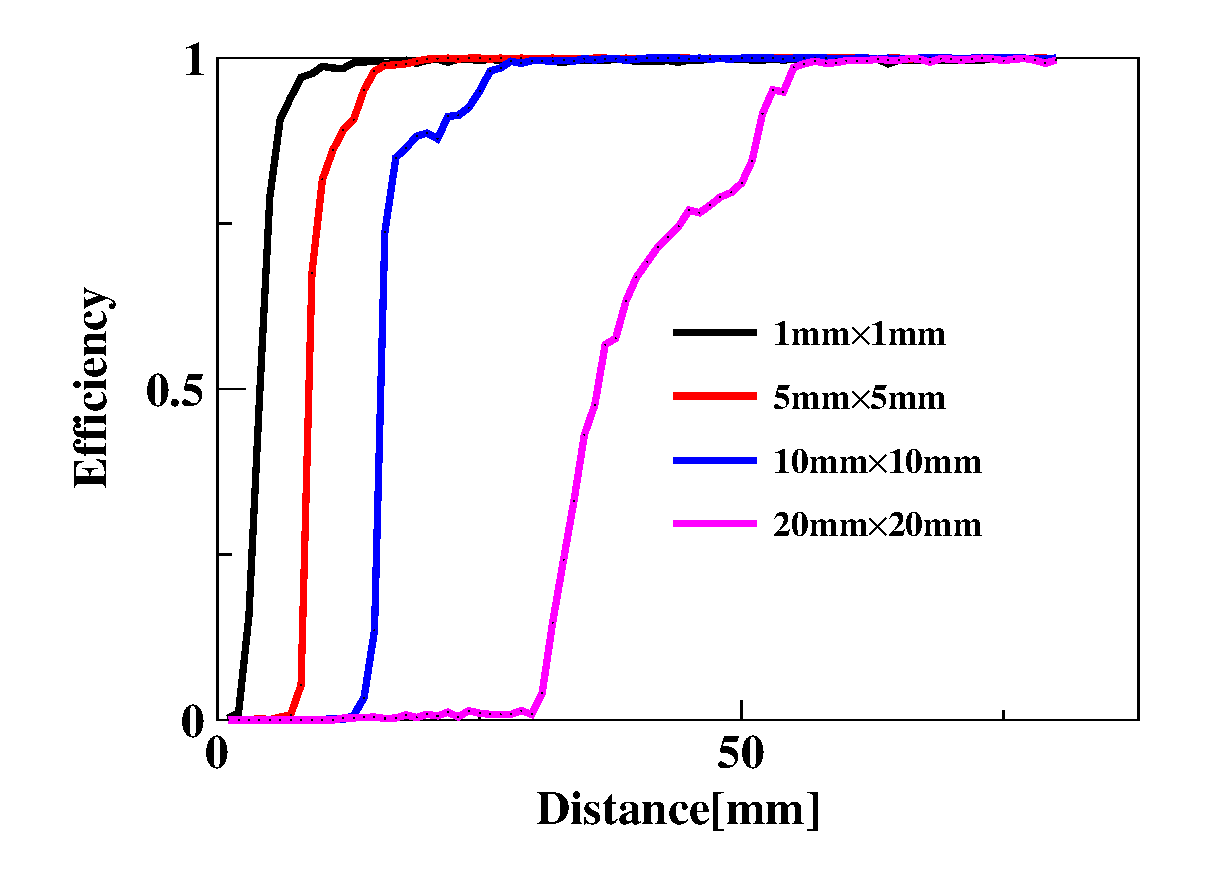
\includegraphics[scale=0.26] {Figures/Performance/zhaohang/SaperationEffeciency}
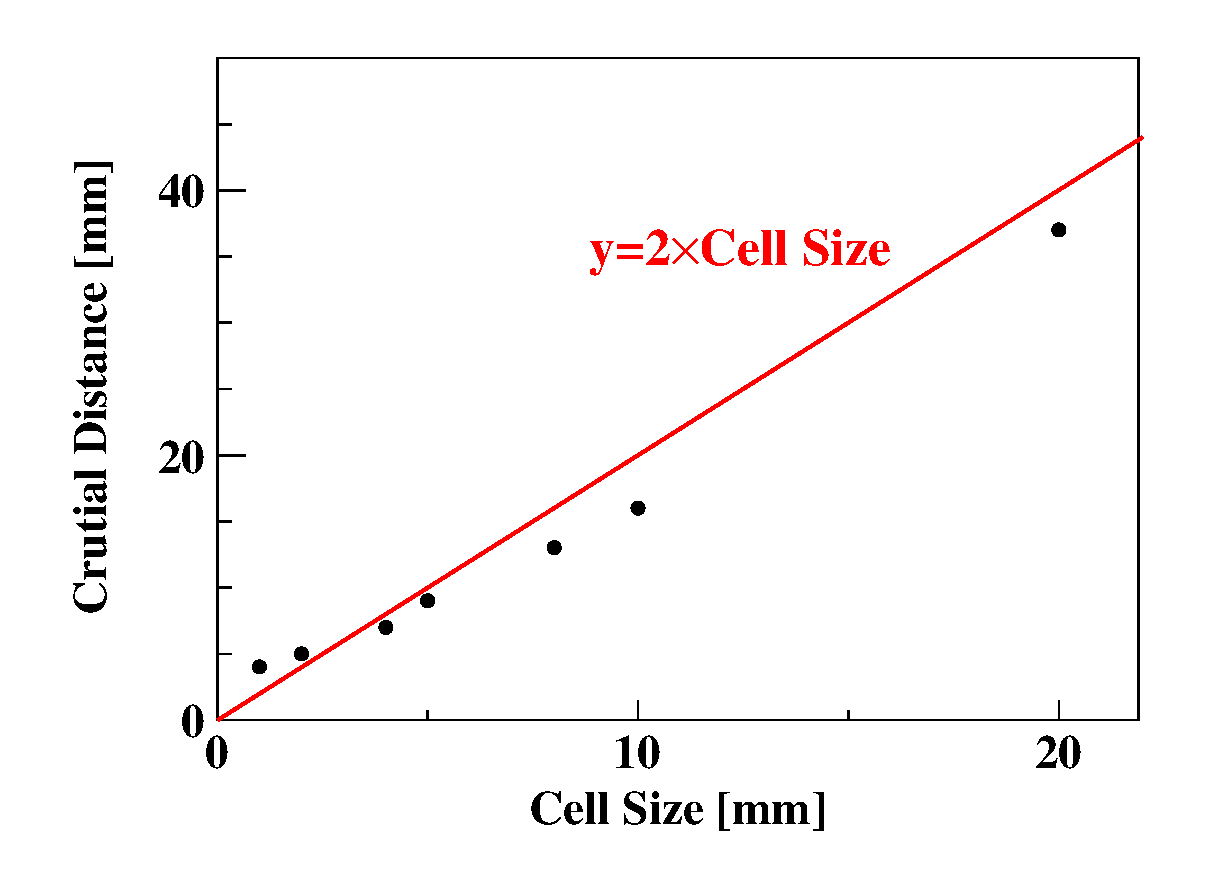
\includegraphics[scale=0.26] {Figures/Performance/zhaohang/SeperationAbility}
\caption{ The separation performance at 2-photon events at different cell sizes.}
\label{fig:seperation}
\end{figure}





To conclude, Arbor is a geometrical algorithm that reconstructs each shower clusters into a tree topology.
At high granularity calorimeter, Arbor allows not only an efficient separation between different particles,
but also leads to a reconstruction of the shower inner structure.
Meanwhile, Arbor maintains a high efficiency in collecting the shower hits/energy,
which is important for the shower energy estimation. 

The overall performance on different physics object and physics benchmarks will be discussed in details in the following sections. 




\section{Leptons}
The lepton identification is of key importance to the CEPC Higgs program.
First of all, about 7\% Higgs boson events at the CEPC are generated together with a pair of leptons.
Those events are the golden signals for the Higgs recoil analysis, which is the anchor for the absolute Higgs measurements.
A significant fraction of the Higgs boson decays,
directly or via cascade, into final states with leptons. 0.02\% of SM Higgs decays into muons;
the leptons serve as the essentially candles of identification of $H\to WW/ZZ\to$ leptonic/semi-leptonic final states.
In addition, a significant fraction of Higgs->bb/cc events generate leptons in their decay cascade. 

The PICADOR detector, especially its calorimeter system, provides enormous information for the lepton identification,
in the sense that a high-energy electron/positron/hadrons is likely to induce thousands
of hits in the calorimeter with typical spatial configurations. Using the benchmark calorimeter geometry,
the shower fractal dimension, a powerful lepton identification variable, could be extracted [Ref FD].
In addition, the dE/dx measured by the TPC could efficiently separate electron/positrons from muon and hadrons,
at track energy less than 10 GeV.
\begin{figure}[h!]
\centering
\includegraphics[scale=0.22]{Figures/Performance/dan/2dlikeness.pdf}
\includegraphics[scale=0.30]{Figures/Performance/dan/eff_ES.pdf}
\caption{Left, calculated lepton likelihood for Electron, Muon and Pions;
  Right, efficiency of muon, electron and pion identifications. }
\label{fig:performance-lepton}
\end{figure}

A dedicated Lepton identification algorithm for the detectors using high granularity calorimeter, LICH [Ref LICH], has been developed.
LICH extract more than 20 distinguish variables from the detector and combine these information into lepton-likelihood via MVA method.
Applied on isolated charged particle candidate with energy larger than 2 GeV,
lepton identification efficiency better than 99.5\% could be achieved with a mis-identification rate from hadrons
is controlled to be smaller than 1\%.
This mis-identification is mainly induced by the irreducible background rate from pion decay (to muons)
and highly electro-magnetic like pion clusters (via the pion0 generated from the pion-nuclear interactions).
Not surprisingly, this performance is significantly better than that at LHC and LEP [Ref XX]. 
In the actual physics event, the lepton identification performance will be limited by the separation power of the particle detector.
As a control sample, we studied the $llH$ event reconstruction
and studied the efficiency of successfully identify two leptons with opposite charge.
The analysis shows that the total event reconstruction efficiency reaches 97-98\%,
which, taken into account the detector acceptance, is slightly degrades from the isolated particle performance,
but highly consistent with Arbor separation power.
In other word, less than 1\% of the objective leptons in the llH events will potentially be mis-identified
due to the overlapping of their cluster to the nearby showers. 

\begin{figure}[h!]
\centering
\includegraphics[scale=0.30]{Figures/Performance/zhenxing/DataRooFitPlotmd.pdf}
\includegraphics[scale=0.30]{Figures/Performance/zhenxing/DataRooFitPlotmi.pdf}
\caption{Reconstructed recoil mass distribution for the $l^+l^-H$ events, the left is for $e^+e^- \to \mu^+\mu^-H$ and the right for  $e^+e^- \to e^+e^-H$  }
\label{fig:performance-llrecoil}
\end{figure}

\section{Kaon Identification}

Successful identification of the charged kaons from other hadrons,
especially from charged pions, allows the tagging to the $s$-quark and is highly appreciated in the flavor physics.
According to the Bethe-Bloch equation, in the realistic energy range
(for example with energy larger than 2 GeV) and at the same track momenta,
the dEdx of pions is larger than that of kaons by roughly 10\%.
In other word, if the dEdx resolution could be measured to a relative accuracy better than 5\%,
the dEdx could leads to an efficient $\pi$-$K$ separation.

The PICADOR detector geometry is equipped with a large TPC main tracker, which is segmented into more than 200 radical.
Depending on the readout hardware performance,
the $dE/dx$ resolution leads to 2-4 $\sigma$ $\pi$-$K$ separation for 2-20 GeV charged tracks.
See the left plot of Fig.~\ref{fig:dedx}. The upper boundary is the ideal separation predicted by the Geant4 simulation;
while the lower boundary includes a conservative estimation on the DAQ procedure.
The $dE/dx$ separation between other charged particles is also demonstrated. 

\begin{figure}[h!]
\centering
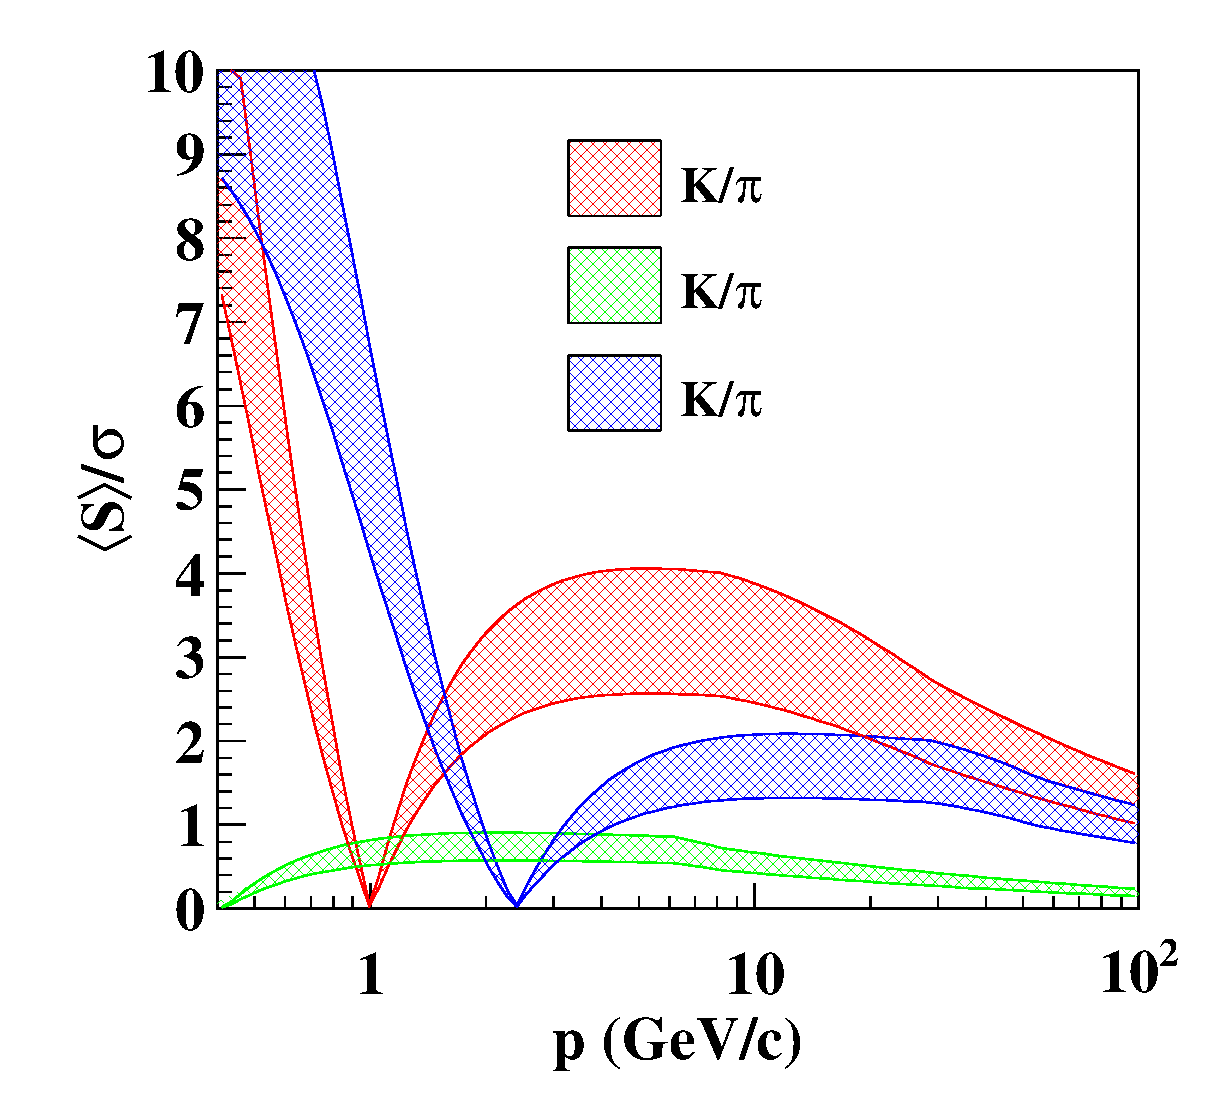
\includegraphics[scale=0.55]{Figures/Performance/anff/sep2p}
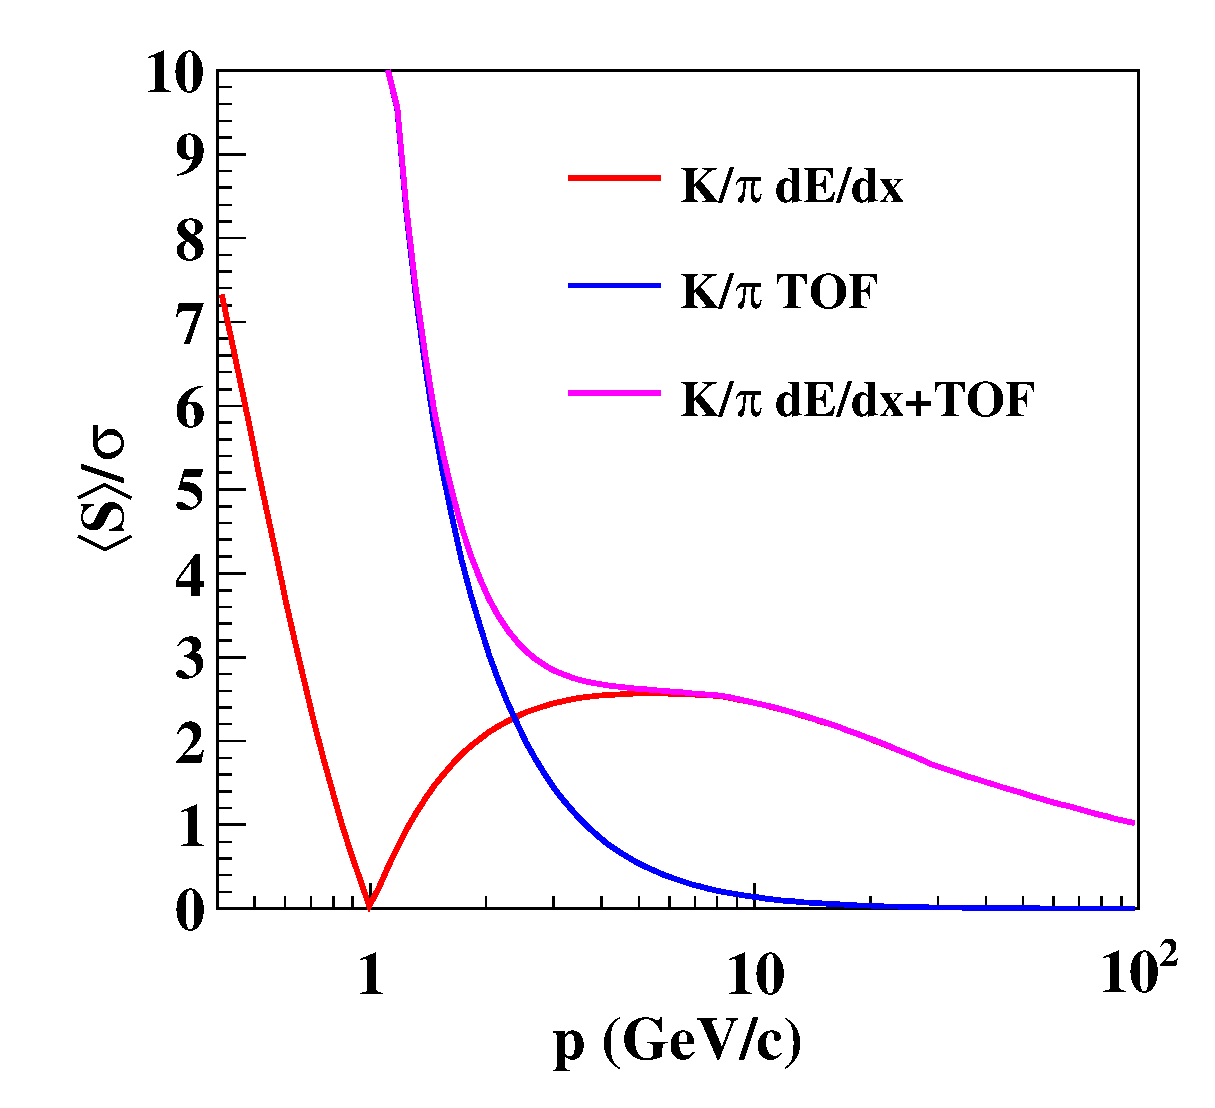
\includegraphics[scale=0.55]{Figures/Performance/anff/sep2p_tof}
\caption{$\pi$-$K$ separation performance at PICADOR detector.
  Left plot, $dE/dx$ separation between different charged particles at $0.4\sim 100$ GeV track momentum.
  Right plot, the separation power using both $dE/dx$ and ToF information.}
\label{fig:dedx}
\end{figure}

The difference between the $dE/dx$ of pions and kaons vanishes at 1 GeV track momentum.
On the other hand, a significant portion of charged particle is at energy lower than 2 GeV.
To ensure the pi-kaon separation performance for these low energy tracks,
a Time of Flight (ToF) measurement is proposed on top of the $dE/dx$ measurement.
The ToF information could be measured by the ECAL, with a few layers equipped with the Time sensitive ASICs.
According to the recent progress of high granularity calorimeters,
an ECAL with 50 ps time resolution is within the current technology reach.
Using both ToF and $dE/dx$ information,
a separation better than 2 $\sigma$ could be achieved for tracks with momenta smaller than 20 GeV. 

Considering the CEPC inclusive $Z\to q\bar{q}$ sample and integrate over the full polar angle and the momenta range of $2\sim 20$ GeV,
an over all kaon identification reaches an efficiency and purity of 90\%/90\%.
This performance could be significantly improved by using more homogenous and more accurate amplification/DAQ system,
and to optimize the TPC geometry by using thinner radical layer and/or larger TPC out radius.
It has been demonstrated that,
a proper combination of the TPC geometry and a sophisticated readout system
could enhance the charged kaon identification performance to an efficiency/purity of 99\%/99\%.

\section{Photons}

A successful reconstruction of photon is crucial for the jet energy measurement,
the $Br(H \to \gamma \gamma)$ measurement and the $\tau$ physics.
The reconstruction of photons could be characterized by its reconstruction efficiency,
its energy resolution and the identification from other neutral objects such as neutrons.  

The reconstruction efficiency of photons certainly depends on the photon energy.
The PICADRO detector is sensitive to photon with energy larger than 10 MeV,
and the reconstruction efficiency saturate close to 100\% for photon energy larger than 1 GeV.
Proportional to the material budget before the calorimeter,
roughly 10\% of the photons at PICADOR convert into $e^+e^-$ pairs or even start an EM showers before reaching the calorimeter.
Thanks to the sophisticated lepton identification performance and the large solid angle coverage,
most of these converted photons could be identified. 
    
The PFA level photon energy reconstruction is depending on the intrinsic ECAL energy resolution
and the PFA algorithm energy collection efficiency and purity.
The energy collection efficiency, or say the hit collection efficiency, is certainly a function of the incident particle energy/type.
Using iterative reconstruction algorithm, Arbor reaches reconstruction efficiency higher than 99.9\%
for photons with energy larger than XX GeV, see also XXX. 

The identification of photons from the neutron background is straight forward.
Combined with the ToF information and the shower profile information,
the identification performance could reach a level such that, at 99.9\% identification efficiency,
the mis-identification rate of neutron to photons is smaller than XX\%.
Meanwhile, the overlapping between photon showers and other particle showers may degrade the identification efficiency,
however, since the PICADO detector has large tracker radius and very high granular ECAL readout cells,
this degrading is limited to sub-percentage level. 

The overall photon reconstruction could be characterized by the $Br(H \to \gamma \gamma)$ measurement.
On the other hand, the photon reconstruction is sensitive to the geometry defects, such as the cracks between ECAL modules,
staves, and the dead zone between ECAL barrel and endcaps.
To benchmark the impact of geometry defects, a simplified,
defect-free ECAL geometry has been implemented into the Geant 4 simulation.
This simplified ECAL uses cylindrical barrel layer and its endcaps is directly attached to the barrel, forming a closed cylinder. 
Fig.~\ref{fig:performance-diphoton} shows the Higgs boson invariant mass reconstructed from $Br(H \to \gamma \gamma)$ signal at a simplified ECal geometry.
A relative signal width of 1.7\% is achieved, which agrees with the intrinsic electron energy resolution,
of 16\%/sqrt(E), measured from the TB data of the Si-W ECAL prototype. 
%
\begin{figure}[h!]
\centering
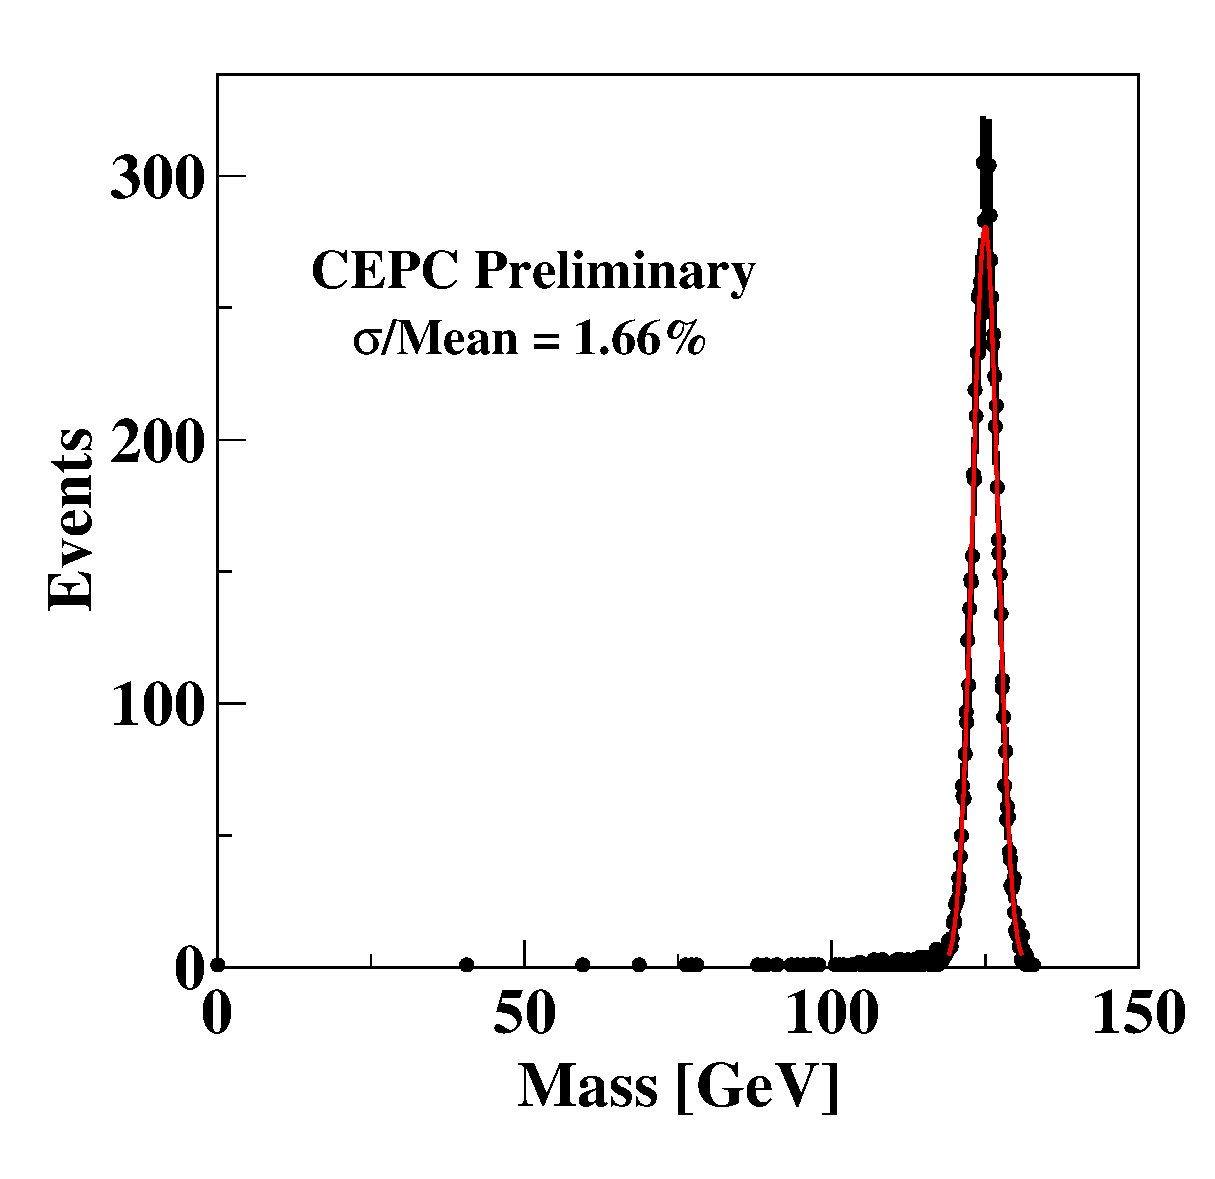
\includegraphics[scale=0.32]{Figures/Performance/zhaohang/h_gammagamma}
\caption{The reconstructed Higgs invariant mass of $H \to \gamma \gamma$ events  }
\label{fig:performance-diphoton}
\end{figure}



The Higgs to di photon signal is also studied at the PICADRO geometry, where a relative signal width of 2.2\% is observed.
This degrading is mainly induced by the geometry defect in between the ECAL module and ECAL staves.
In addition, the impact of detector inhomogeneity and detector dead zones is also studied,
where both effects causes significant degrading to the Higgs mass resolution via H->gammagmma events. 


\section{Taus}

$\tau$'s are extremely intriguing physics objects.
As the heaviest lepton in the SM, a significant fraction of the SM Higgs boson decays into di-tau final states.
As a result, g(Htautau) is anticipated to be measured better than 1\% relative accuracy at the CEPC.
Measuring the polarization of Tau at the $Z$ pole leads to a precise determination of Afb(tau) and therefore $\sin^2\theta$.
The reconstructions of tau functional spectral is of key importance to the CEPC EW program,
as it grant the access to a precise reconstruction of $\alpha_S$, XX, EW parameters. 

A successful reconstruction of the tau lepton is not a trivial task, for the tau lepton has various decay final states.
In the CEPC collision environment, we catalog the tau events into two catalogues according to the event topology,
and the reconstruction algorithm and performances has been studied respectively. 

The first catalogue is the leptonic catalogue, where no physics objects,
or only lepton/photon/Missing energy momentum is generated together with the tau candidates.
These events include, for example: 

\begin{itemize}
\item[]1, $e^+e^- \to ZH, Z\to ll$ or $\nu\bar{\nu}, H \to \tau^+\tau^-$ events;

\item[]2, $e^+e^- \to ZZ \to ll/\nu\bar{\nu} + \tau^+\tau^-$ events;

\item[]3, $WW$ events with $l\nu \tau\nu$ final states;

\item[]3, ISR return events at Higgs runs, with $Z$ decays into a pair of $\tau$'s; 

\item[]4, $Z \to\tau^+\tau^-$ events at CEPC $Z$ pole operation. 

\end{itemize}

A successful identification of these events based highly on the reconstruction of photons and charged hadrons. 

The second catalog is the hadronic catalog, where the tau pairs is generated with jets. For instance, we have: 

\begin{itemize}
\item[]1, $ZH, Z \to qq, H \to \tau\tau$

\item[]2, $ZZ \to qq \tau\tau$

\item[]3, $WW \to qq \tau\nu$

\item[]4, $ZH, Z->qq, H \to WW \to l\nu \tau\nu$
\end{itemize}


To find the tau lepton in the hadronic catalog is much more challenge than that in the leptonic environments.
The identification algorithm would always be a compromise between the signal efficiency and purity. 

The performance of the first catalogue could be represented by the $Br(H\to\tau^+\tau^-)$ measurement at $\mu^+\mu^- H$.
The inclusive SM background could be efficiently subtracted by requesting the proper number of lepton
and limit the number of photon and charged hadrons.
The background reduction could be further enhanced by restrictions on the recoil mass against the muon system.
To further suppress the remaining background,
the BDT method that combines the kinematic information from tau candidates has been applied.
The pull of impact parameter of the leading track in the tau candidates has been shown in the left plot of Fig.~\ref{fig:tautau},
where the signal is clearly separated from the background. 

Thanks to the precise reconstruction of leptons, photons and charged hadrons,
the final event selection efficiency of $\mu^+\mu^-H$ events is 93\%
and the entire SM background is controlled to a statistic smaller than the signal ---
in other word, suppressed by nearly 6 orders of magnitudes.
It should be noticed that the leading remaining background is the irreducible Higgs background from Higgs to $WW$ decays.
A relative accuracy of 2.7\% is achieved for the signal strength measurement in the $\mu^+\mu^- H$ channel. 

\begin{figure}[h!]
\centering
\includegraphics[scale=0.30]{Figures/Performance/dan/newe2e2H.pdf}
\includegraphics[scale=0.30]{Figures/Performance/dan/newqqH.pdf}
\caption{The pull of impact parameters at $Br(H \to \tau^+\tau^-)$ measurement via $\mu^+\mu^-H$ (left) and $q\bar{q}H$ channel(right). }
\label{fig:tautau}
\end{figure}


The second catalogue includes the tau reconstruction at $q\bar{q}H$, Higgs->tautau events.
A double size cone-based tau tagging algorithm has been developed.
Two cones at different sizes are scanned for each individual track.
The cone parameters, including the sizes, the invariant mass, and the energy ratios,
are optimized toward the objective measurement.
In short, by requesting two tau candidates with opposite charge,
the signal efficiency is 57\% and the background could be suppressed by 3 orders of magnitude.
Following a similar BDT event selections as in the mumuH analysis, the pull of the impact parameters has been extracted,
see the right panel of Fig.~\ref{fig:tautau} A relative accuracy of 1.7\% is achieved in the $q\bar{q}H$ channel [ref. DanNote]. 

To conclude, the tau reconstruction at the CEPC is currently catalogued into leptonic and hadronic events
and reconstructed using different strategy and tau finding algorithm.
In the leptonic events, the tau events identification relies strongly on a successful reconstruction of the photons,
charged hadrons and leptons.
Since the CEPC reference detector ensures a powerful particle flow reconstruction of these final state particle,
the tau candidate identification reaches almost an ideal efficiency and purity.
In the hadronic events, cone-based tau-tagging algorithm has been developed,
which could reach an efficiency/purity better than 70\%/70\%.
In both cases, a precise reconstruction of the impact parameter --- the pull from the IP ---
plays an important role in the tau events identification.  

It should be emphasized that the physics requirements arisen from the tau physics is more demanding
than the $Br(H\to\tau^+\tau^-)$ measurements.
The former request an clear separation between the photons generated from $\pi^0$ in the $\tau$ decay cascade,
while the latter only request a clear separation between signal and backgrounds. 



\section{Jet-clustering\label{sec:jet-clustering}}
The jet reconstruction is crucial to the CEPC physics program.
Since roughly 60\% of the jet energy is stored in charged hadrons,
whose momentum is usually measured at a superior precision in the tracker than in the calorimeter.
Therefore, Particle Flow Algorithms could improve significantly the precision of jet energy measurement,
with respect to the calorimeter only reconstruction. 

At CEPC reconstruction, the jet candidates are clustered from the reconstructed particles.
The ambiguities from the jet clustering, i.e, wrongly grouping of the final state particle,
could be a significant effect and need careful investigation. To characterize the jet reconstruction performance,
a two-stage analysis has been performed on the following samples: 

\begin{itemize}
\item [] 1, $\nu\nu qq$ events via the $ZZ$ intermediate state;

\item [] 2, $l\nu qq$ events via mostly $WW$ intermediate state;

\item [] 3, $\nu\nu H$ events with $H \to b\bar{b}, c\bar{c},~\mbox{or}~gg$;
\end{itemize}

The first stage is the boson mass reconstruction.
In these events, despite possibly one isolated lepton (in WW events) and isolated ISR photon(s),
all the final state particles are decayed from one individual massive boson.
Therefore, no jet clustering algorithm is needed and the boson mass could be reconstructed directly
from all the visible final state particles. 

A second stage analysis is applied on the jet candidates.
Vetoing the isolated photon and leptons,
we forced the remaining final state particle into 2 reconstructed jets via the ee-anti-kt algorithm (Reco-Jets).
The same jet-clustering algorithm is also applied to the final state particles at the generator level,
and forming the Gen-Jets.
Therefore, the energy/angular responses could be studied via the comparison of initial quarks,
the Gen-Jets and the Reco-Jets.
Clearly, the difference between the initial quarks and Gen-jets is stemmed from the fragmentation and jet-clustering algorithm,
while the difference between Gen-jets and Reco-jets includes the detector performances. 

The result of the first stage study is shown in Fig.~\ref{fig:jet-HZW},
which displays the reconstructed invariant mass spectra of all the final state particles except the possible isolated lepton.
Clearly, each histogram exhibits a significant mass peak at the anticipated position.
Meanwhile, various physics effects exhibit in these corresponding plots, lead to a wider distribution:

\begin{itemize}
\item[] 1, In the $\nu\nu qq$ events, most of the jets decay from a on-shell $Z$ boson, however,
  the $Z-\gamma$ interferences give rises to a low energy plateau. 

\item[] 2, All the mass peaks exhibit a clear high mass tail, induced by the ISR photon.
  In the $l\nu qq$ events, the high mass tail is also induced by the physics processes
  where the final states jets is not decayed from a intermediate W boson.

\item[] 3, Low mass tails induced by the neutrinos generated in the heavy flavor jet decay cascade
  (i.e, $W \to cs, Z/H \to cc~\mbox{or}~bb$). 
\end{itemize}

To disentangle these physics effects from the detector response,
we restrict the samples by vetoing the heavy flavor jets (in the middle raw of Fig.~\ref{fig:jet-HZW})
and by additionally veto events with significant ISR photons (in the lower raw).
Clearly, the peaks become much narrower after applying those cuts.

%
\begin{figure}[h!]
\centering
\includegraphics[scale=0.56]{Figures/Performance/peizhu/HZW_mass_withoutGrid9.pdf}
\caption{ Reconstructed boson masses from physics benchmarks of $\nu\nu qq$ events (left), lvqq events(middle) and vvH, H->qq events (right). The raws are corresponding to inclusive samples, light flavor samples and light flavor + ISR cleaned samples.  }
\label{fig:jet-HZW}
\end{figure}



\begin{figure}[h!]
\centering
\includegraphics[scale=0.30]{Figures/Performance/peizhu/HZW_mass_withoutGrid1.pdf}
\includegraphics[scale=0.30]{Figures/Performance/peizhu/HZW_mass_withoutGrid5.pdf}
\caption{Overlapped PDFs from reconstructed 2-jets events. Left: inclusive samples; right, cleaned samples. }
\label{fig:jet-three-peaks}
\end{figure}


After these cleaning, a relative resolution of 3.8\% is reached for the Higgs invariant mass reconstruction
via $\nu\nu H, H\to gg$ events.
Giving the fact that the SM Higgs boson has a width of 4.2 MeV, this accuracy is mainly induced by the detector resolution.
Similar level of Boson mass resolution is achieved for $W$ and $Z$ boson
once the intrinsic boson mass width is deconvoluted from the overall distribution.
Therefore, we conclude that the boson invariant mass could be measured to better than 4\% at this CEPC reference detector. 

Fig.~\ref{fig:jet-three-peaks} shows the overlapped PDFs extracted from Fig.~\ref{fig:jet-HZW}, each normalized to a unit area.
The left/right plot is corresponding to the inclusive/cleaned samples accordingly.
A clear separation between the mass peak of $W$, $Z$ and Higgs boson exhibits for both plots, meanwhile,
cleaning the heavy flavor and ISR events significantly enhances the separation. 

The second stage analysis is applied on the vvqq sample. The entire visible energy/momenta was clustered into 2 jets. These 2 jets are classified into leading/sub-leading jets according to their energy. The jet energy scale (JES) and jet energy resolution (JER), defined as the relative differences between the Genjet and the Recojet, has analyzed accordingly. The relative energy difference between the RecoJet and GenJet could be modeled by a core function (double sided crystal ball) convoluted with a Guassian. The core function is induced mainly due to the jet clustering and detector acceptance effects, while the Guassian described the detector resolution. The mean value of the Gaussian is defined as the JES while the relative width of the Guassian is defined as the jet energy resolution (JER).

\begin{figure}[h!]
\centering
\includegraphics[scale=0.30]{Figures/Performance/peizhu/ROOTFit_RecoMCP_VS_bin7.pdf}
\includegraphics[scale=0.30]{Figures/Performance/peizhu/ROOTFit_RecoMCP_VS_bin8.pdf}
\caption{jet energy scale as a function of the jet directions. }
\label{fig:jet-energy-scale}
\end{figure}
Fig.~\ref{fig:jet-energy-scale} shows the JES at different jet directions for both jets.
The entire amplitude of the JES is controlled to 1\% level,
which is roughly 1 order of magnitude better than that at LHC.
The JES is completely flat along the azimuth angle.
Along the polar angle, the JES increases significantly for the leading jets in the overlap part between endcap and barrel.
Meanwhile, the JES is also larger in the endcap than in the barrel.
One possible explanation is that the Particle Flow confusion terms,
especially the artificial splitting of the charged clusters, increases in these parts.
 
It's interesting to see that the Leading jets has a systematically higher jet energy scale comparing to the sub-leading one,
mainly due to the fact that the classification method is energy, thus jet energy scale dependent.
This effect may well be jet-clustering algorithm dependent. 

\begin{figure}[h!]
\centering
\includegraphics[scale=0.30]{Figures/Performance/peizhu/Compare_CMS2.pdf}
\includegraphics[scale=0.30]{Figures/Performance/peizhu/Compare_CMS3.pdf}
\caption{The jet energy resolution for leading (Left) and sub-leading jets (Right),
  as a function of the jet transverse momenta. The performance at CMS has been overlapped for a reference of comparison.  }
\label{fig:jet-comparision}
\end{figure}



The jet energy resolution (JER) performance for jet with different transverse momenta is displayed in Fig.~\ref{fig:jet-comparision}.
The overall JER takes a value between 6\% (at $P_t < 20$ GeV) to 3\% (at $P_t > 100$ GeV).
The leading jets usually takes a slightly better JER comparing to the sub-leading ones.
Taking the performance of the CMS detector as a reference,
the JER at the CEPC reference detector is 2-4 times better in the corresponding $P_t$ range. 

To conclude, the jet energy response has been analyzed at both boson mass level and at individual jets.
For physics events with one massive boson decays into jet final states,
the boson mass could be measured to a relative accuracy better than 4\% at the PICADOR.
This resolution ensures a significant separation between the $W$ boson, $Z$ boson,
and the Higgs boson at the inclusive physics samples;
despite the separation is significantly limited by various physics effects.
At individual jets, the JES is controlled to 1\% level, which is one order of magnitude better than that of LHC experiments.
The JER is superior by 2-4 times better than the LHC results. 

This superior performance is based on the clean collision environment at the electron positron collider,
and also on the development of detector design and reconstruction efforts.
It not only secures the Higgs property measurements, but also is highly appreciated in the EW measurements.
For instance, this mass separation benefits the Triplet Gauge Boson Coupling (TGG) measurement
in the semi-leptonic channel ($e^+e^- \to WW\to l\nu qq$ and $e^+e^-\to ZZ\to llqq, \nu\nu qq$),
for the reconstructed masses provide separation power on top of the lepton reconstruction.

It should be emphasized that the jet-clustering algorithm has a strong and even dominant impact
in jet reconstruction. Dedicated studies are required to search for the most suited jet clustering algorithm
and the corresponding set up, especially for the 4-jets or even 6-jets events. 

%\section{METs}

\section{Jet flavor tagging}

Identification of jet flavor, such as $b$, $c$, $u/d/s$, and gluon plays an important role in the event reconstruction
and essentially for the measurement of the couplings of the $H \to b\bar{b}, c\bar{c}$, and $gg$,
as well as those of $R_{b/c}$ of $Z$ decays at the CEPC.
Bottom jets can be identified by the fact that bottom quarks form hadrons which have specific masses
and prolonged lifetimes compared to jets formed from lighter quarks.
Charged tracks decaying from bottom hadrons tend to have sizable impact parameters measured with respect to the primary vertex.
If there are two or more tracks originating from the same hadron, its decay vertex can be reconstructed directly.
Bottom jets can be identified if the distance between the primary vertex and the decay vertex is sufficiently large,
and that the reconstructed mass from the combination of the charged tracks is consistent with that of a hadron containing a bottom quark.
The identification of bottom jets based on the impact parameter of charged tracks and information
about secondary vertices has been an essential tool in the event reconstruction of recent energy-frontier collider experiments.
The flavor tagging algorithm of the CEPC benefits from the excellent vertex measurement, 
as well as the PFA oriented design concept, which ensure a very good secondary vertex reconstruction and jet energy resolution.    
Recently, the identification of the charm $c$ jet has also become a target of study with the planning of future $e^+e^-$ colliders,
such as the ILC and the CLIC.
The capability of $c$ jet identification allows us to probe the complete hadronic decays of the Higgs boson $H\to b\bar{b}, c\bar{c}, gg$
as well as flavor-changing neutral currents in the top sector such as $t \to cZ$ and $t \to cH$.
Since charm hadrons have smaller masses and shorter lifetimes compared to bottom hadrons, charm hadrons are more difficult to identify.
Fortunately, the excellent point resolution in the vertex detectors to be employed by future $e^+e^-$ linear colliders makes it possible.

\subsection{Base line}

The LCFIPlus package~\cite{Suehara:2015ura} is used for secondary vertex reconstruction, jet-clustering, and flavor tagging.
The LCFIPlus employs the Boosted Decision Tree (BDT) in TMVA~\cite{Therhaag:2010zz} to do the flavor tagging.
This is a machine learning appoach and based on dedicated training samples, which may be from data or Monte Carlo simulation.  
Roughly 60 variables of each jet are used and all  jets are categorzied into four according to the number of vertex reconstructed.
Each category has its own independent TMVA application.


The CEPC as a Higgs factory is also planned to run at $Z$-pole, and a huge statistics of $Z$ sample will be accumulated,
which can be used for the detector calibration and alignment, 
and as the control sample for systematic uncertainty control.
The data sample of $Z$ pole also provides a set of large statistics and pure training samples for flavor tagging application. 

\begin{figure}[h!]
\centering
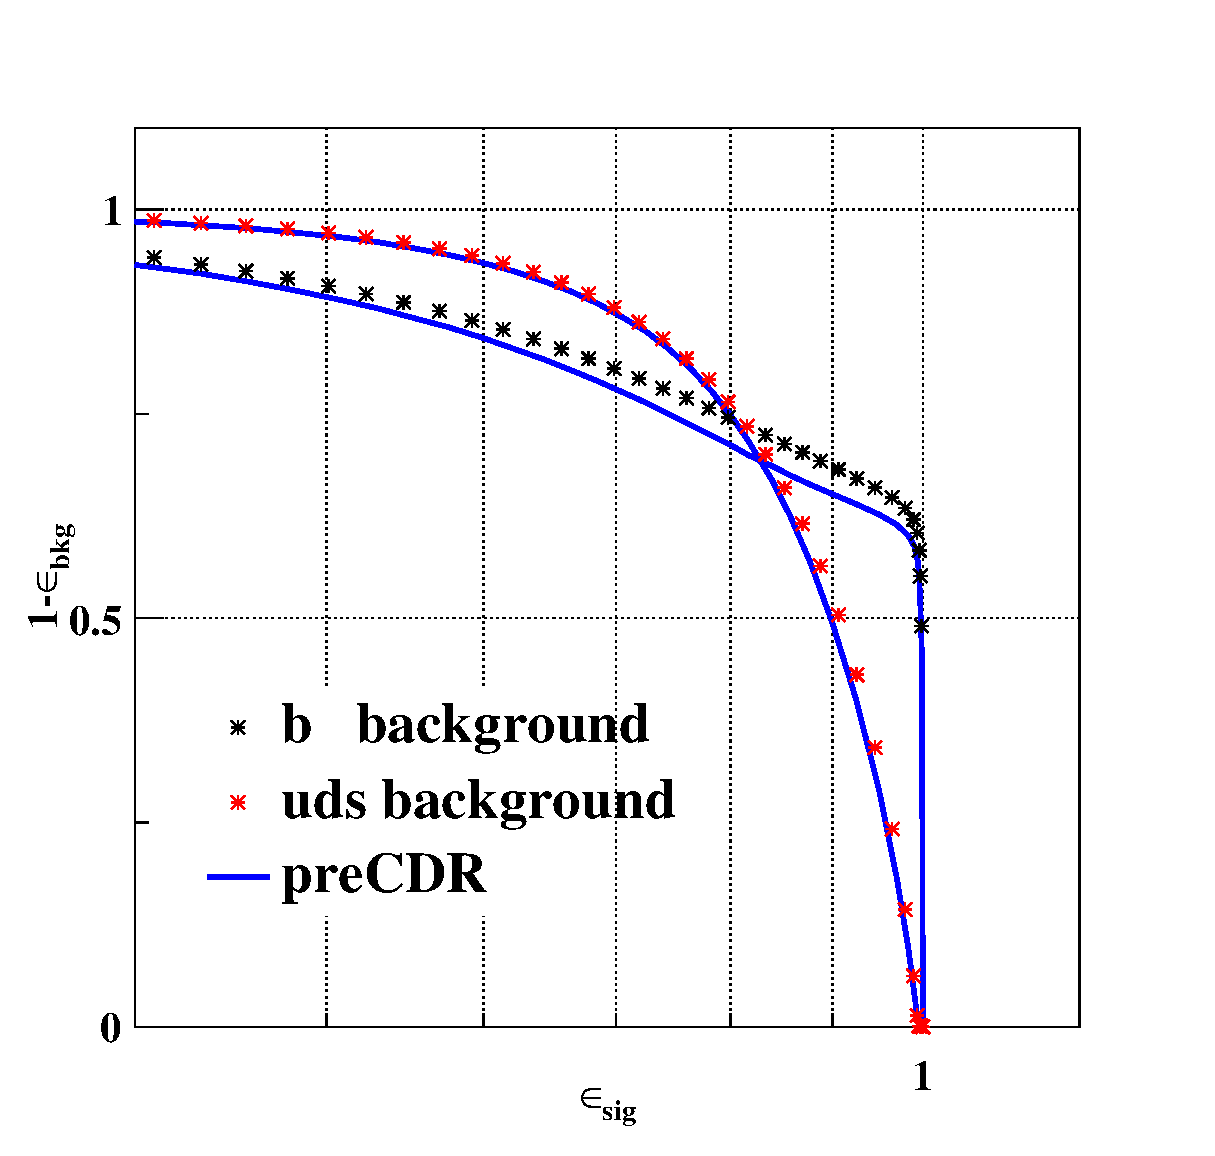
\includegraphics[scale=0.40]{Figures/Performance/ft/CROC-test}
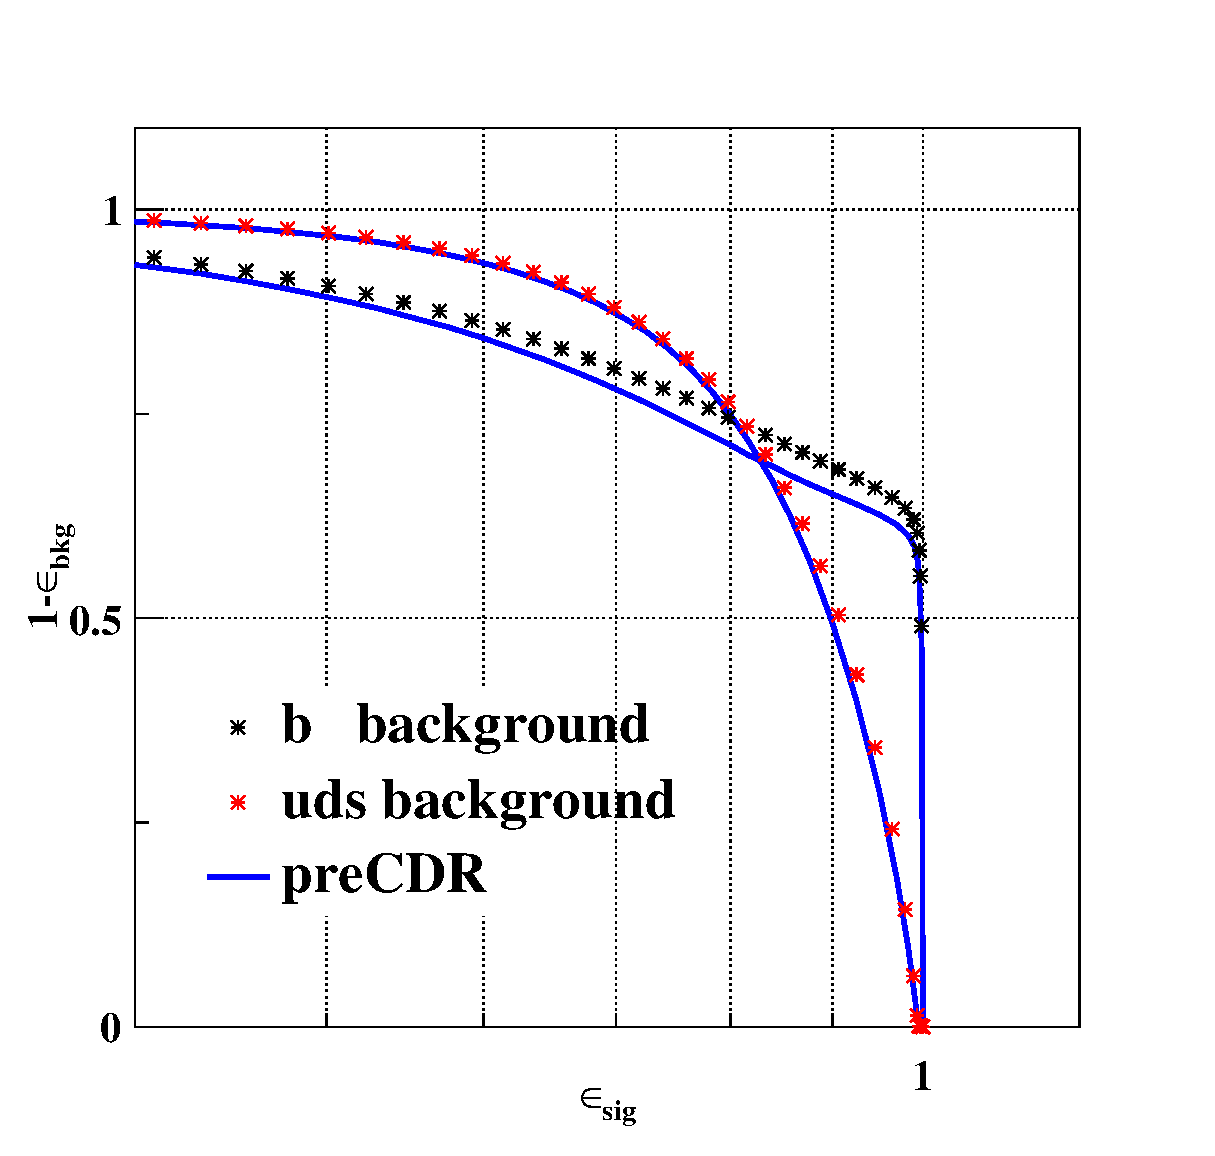
\includegraphics[scale=0.40]{Figures/Performance/ft/CROC-test}
\caption{The Receiver operating characteristic (ROC) curve of $b/c$-tagging shows the performances of flavor tagging compared with those of preCDR.  }
\label{fig:ft-roc}
\end{figure}

\begin{figure}[h!]
\centering
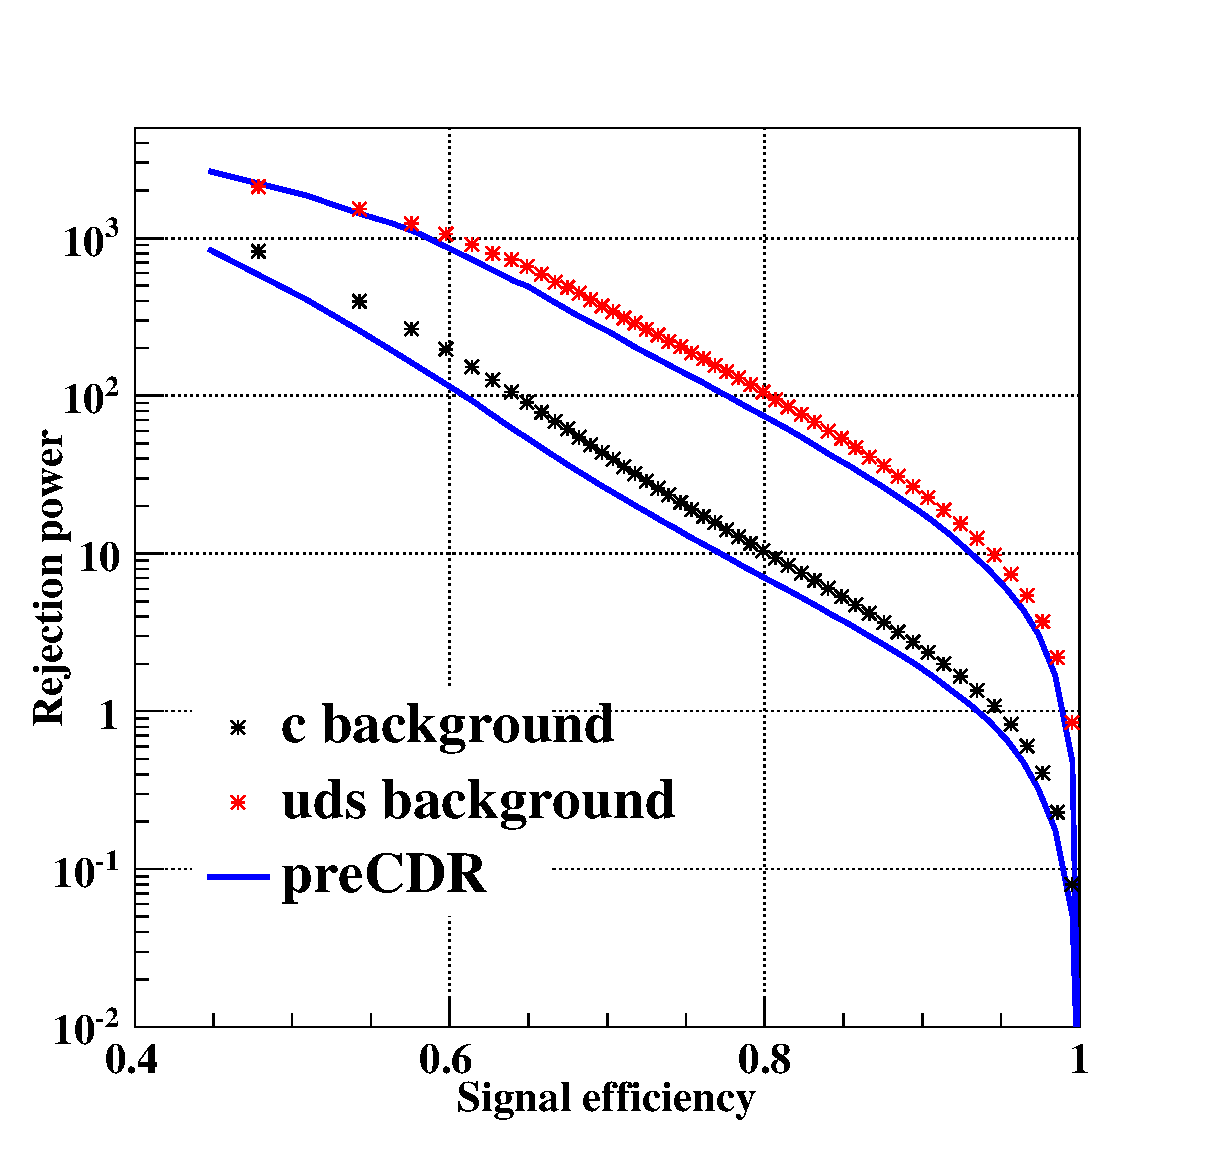
\includegraphics[scale=0.40]{Figures/Performance/ft/rejectionB-test}
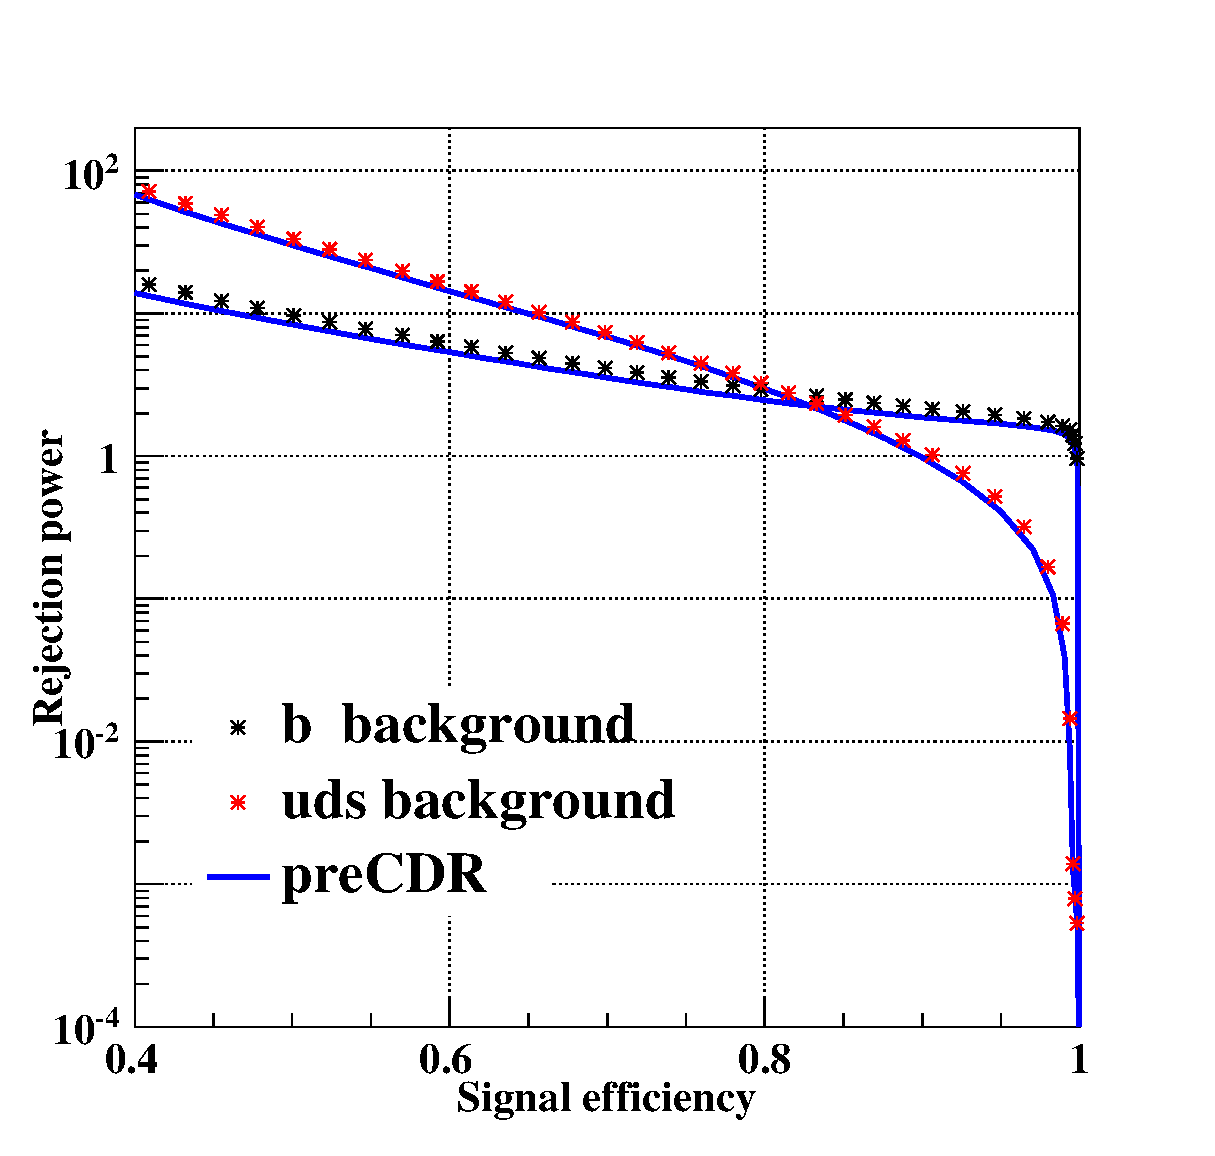
\includegraphics[scale=0.40]{Figures/Performance/ft/rejectionC-test}
\caption{The rejection power vs signal efficiency curves of $b/c$-tagging compared with those of preCDR.  }
\label{fig:ft-rej}
\end{figure}


\subsection{Deep learning}

\subsection{Gluon identification}

\subsection{Geometry scan \& recommendations}

Conclusion;



\bibliographystyle{Style/atlasnote} %% plain.bst
\bibliography{Chapters/Performance} 
